\subsection{Data Balancing}\label{chp3-subsec5}
As noted before in Sect.~\ref{sec:chp2-sec5}, medical data, similar to other real datasets, face the class imbalance problem, and melanoma datasets are not an exception.
Fig.~\ref{fig:dermoscopy_Sens_PerformanceComparison} clearly demonstrates this fact.
Our literature study showed that despite extensive research in melanoma classification, only a few studies tackled the issue of an imbalanced dataset~\cite{barata2013two,celebi2007methodological}.
Barata~\emph{et al.} generated new synthetic samples by adding Gaussian noise with fixed parameters to the minority class samples~\cite{barata2013two}.
Celebi~\emph{et al.} and Capdehourat~\emph{et al.} over-sampled their dataset using \ac{smote}~\cite{chawla2002smote} to improve the \ac{se} of their algorithm~\cite{celebi2007methodological, capdehourat2009pigmented}.
We are convinced that this is an important step, and the effect of imbalanced data on the classification result should be considered.
Therefore, we first balance the majority to a minority class ratio in the data space, and then explore the balancing strategies in the feature space (Sect.~\ref{sec:chp2-sec5}).

\subsubsection{Data space over sampling \acs{dos}}
These methods are related to the generation of new synthetic samples by modifying the original data before doing any feature extraction processes. 
\Ac{dos} is performed on the original dataset by generating synthetic melanoma images based on the two types of deformation:
\begin{description}
	\item[\Ac{rdgm}]. Achieved by adding a random Gaussian motion $\mathcal{N}(\mu, \sigma) = (0,5)$ at each pixel compounded with a global rotation of~\SI{80}{\degree}.
	\item[\Ac{bd}]. Corresponds to a deformation of the original image using barrel distortion compounded with a global rotation of~\SI{145}{\degree}.
\end{description}
\noindent These deformations are used because they are more likely to occur due to a non-planar surface of some body parts, skin wrinkles, and camera orientation. 
Furthermore, cubic b-spline interpolation is used with both methods to approximate non-integer points in the images. 
A synthetic example illustrating the results of these deformations is shown in Fig.\,\ref{fig:DSOS}.

\begin{figure}
  \hspace*{\fill}
  \subfloat[][]{
    \label{fig:GridOriginal}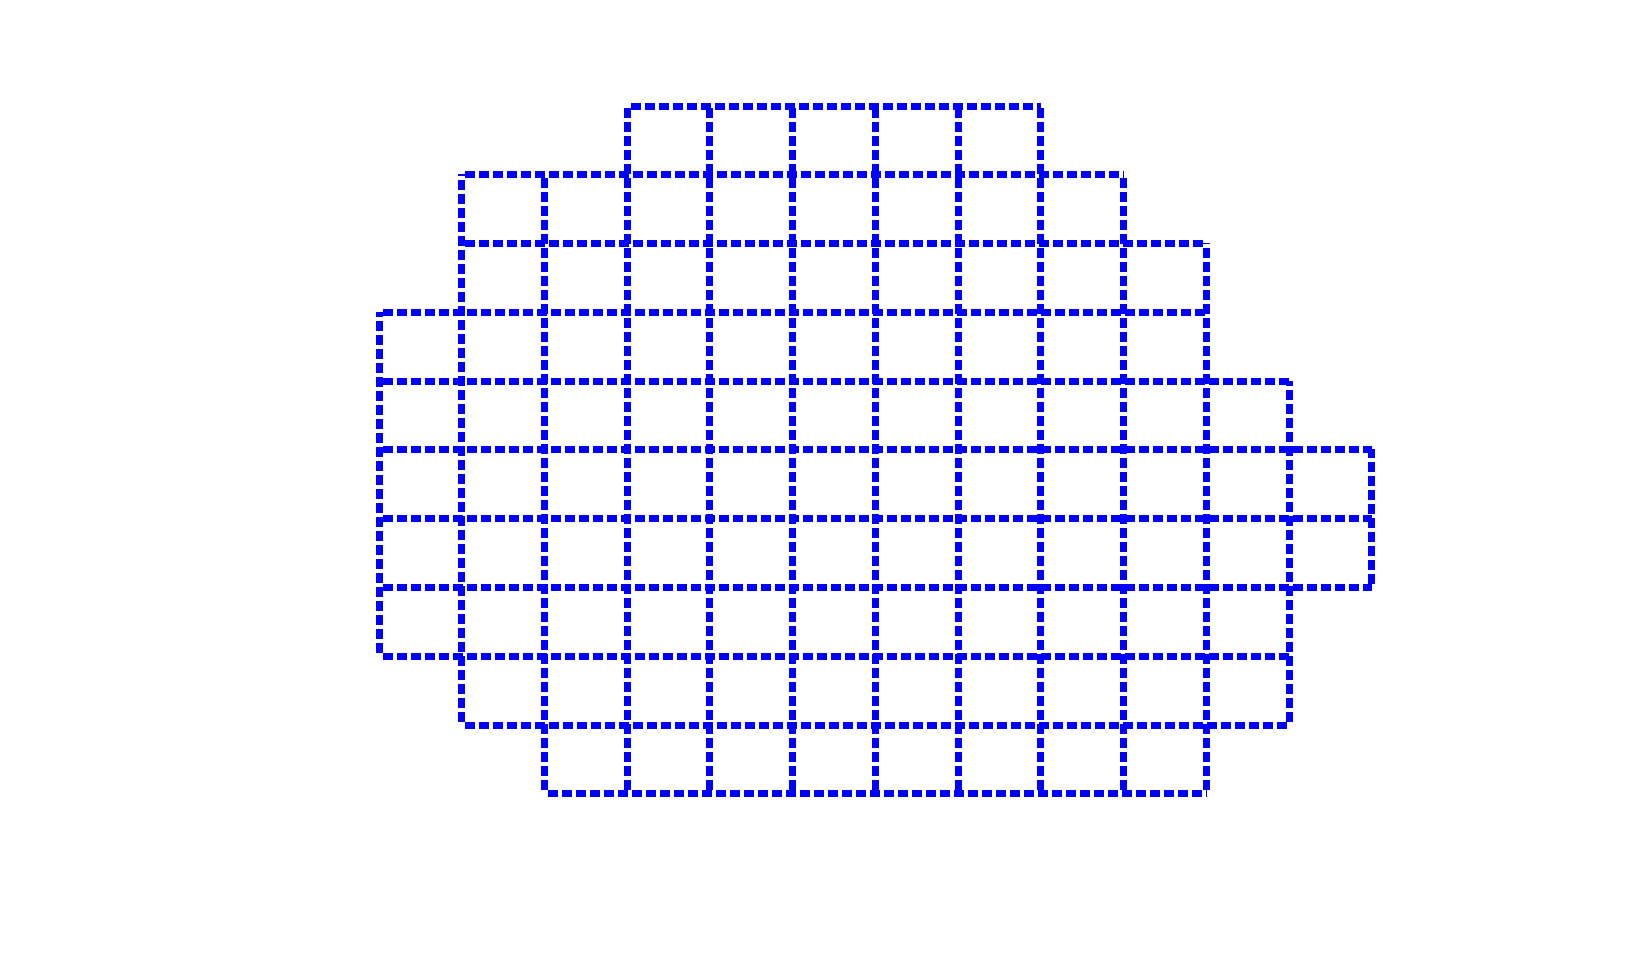
\includegraphics[width=0.3\textwidth]{Chapter3/Figures/OG.png}}\hfill
  \subfloat[][]{
    \label{fig:GridGaussian}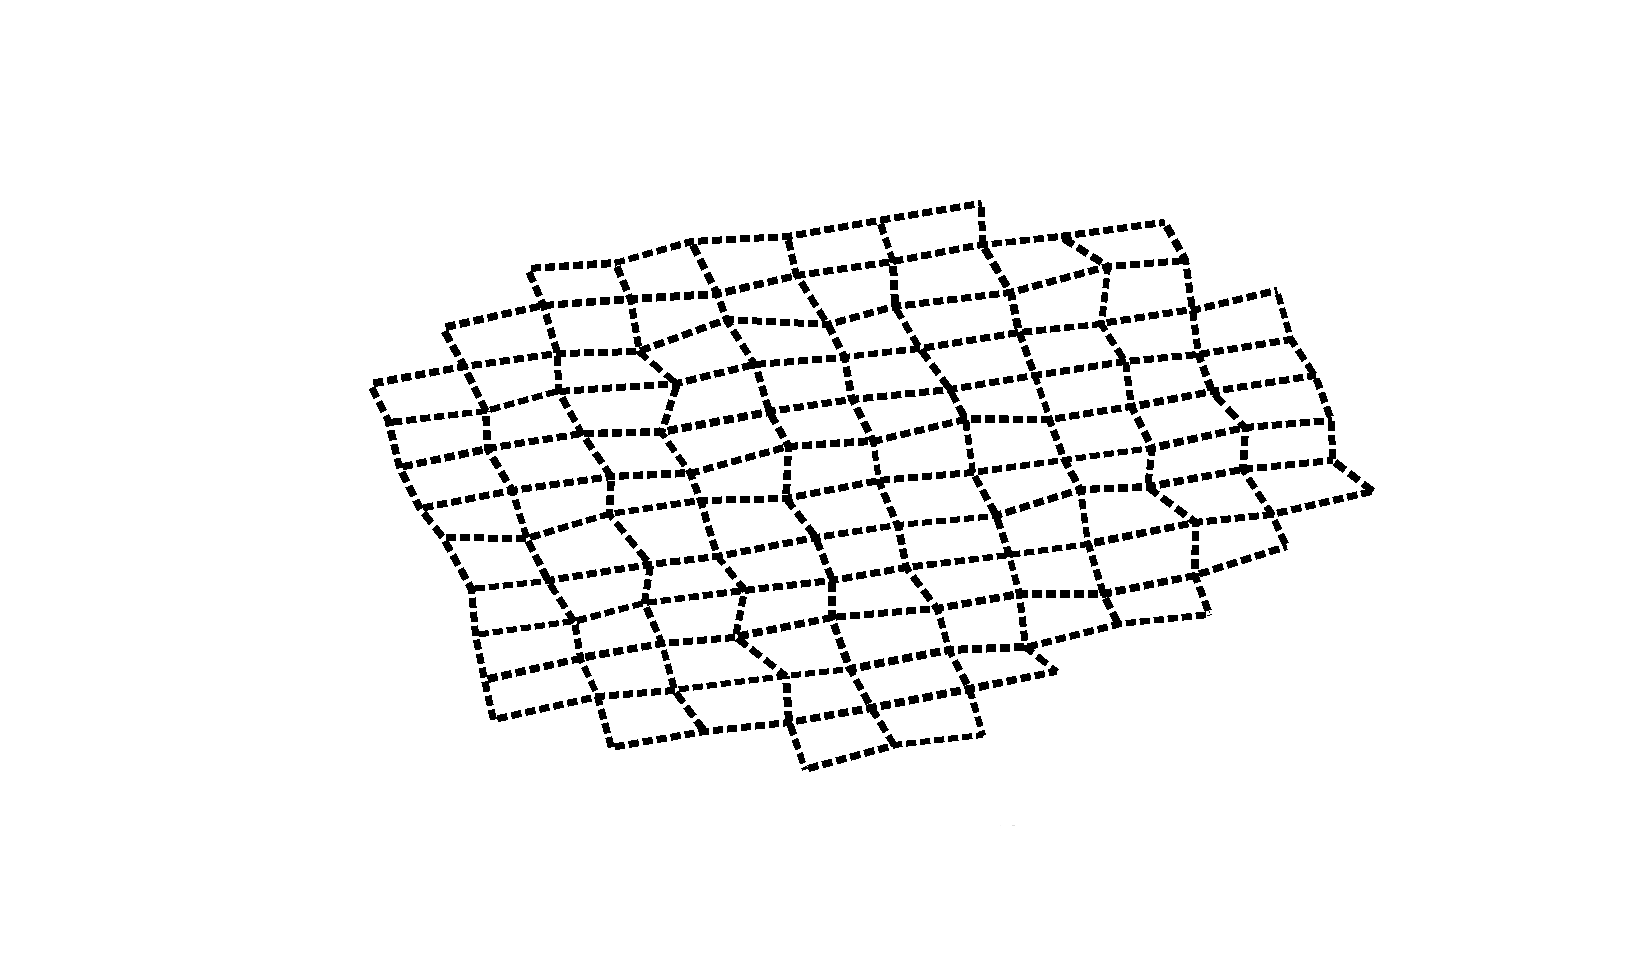
\includegraphics[width=0.3\textwidth]{Chapter3/Figures/GG3_80.png}}\hfill
  \subfloat[][]{
    \label{fig:GridBarrel}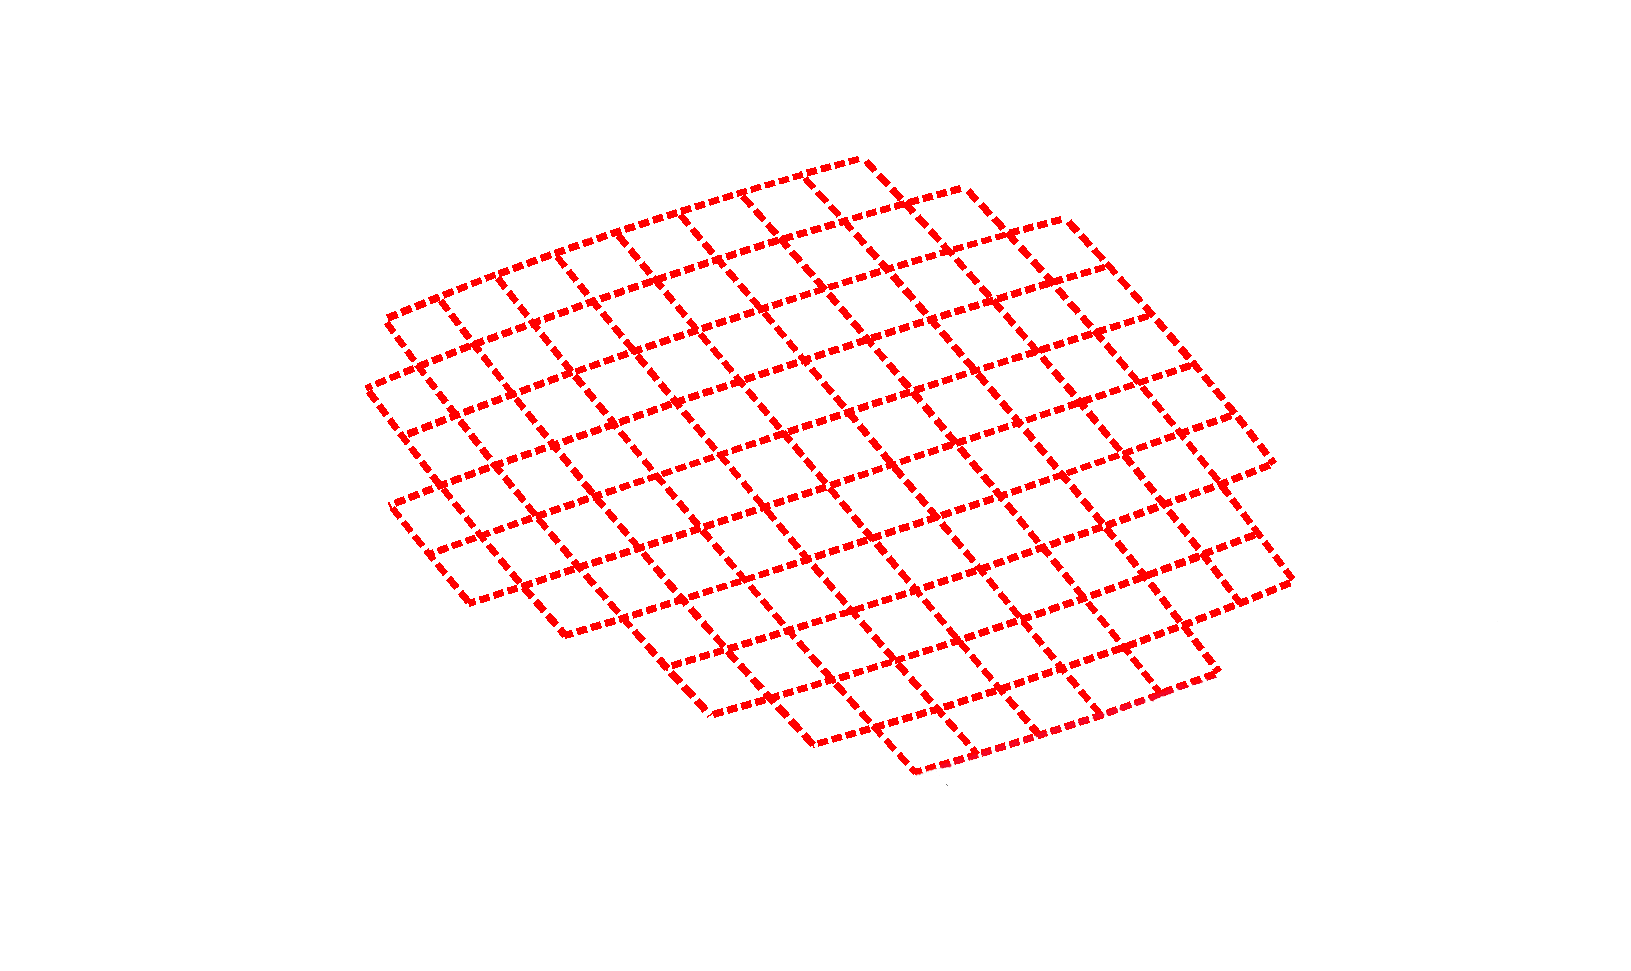
\includegraphics[width=0.3\textwidth]{Chapter3/Figures/BG3_145.png}}
  \hspace*{\fill}
  \caption[Data space over sampling algorithm]{Data space transformation: \protect\subref{fig:GridOriginal} original synthetic data, \protect\subref{fig:GridGaussian} \acs*{rdgm} deformation, \protect\subref{fig:GridBarrel} \acs*{bd} deformation.}
  \label{fig:DSOS}
\end{figure}

\subsubsection{Feature space (over/under)-sampling}
These strategies are discussed extensively in Sect.~\ref{sec:chp2-sec5}.
%Obviously in these strategies the sampling is performed in feature space.
In the over-sampling approaches, such as \ac{smote} and \ac{ros}, minority samples are selected or synthetically generated to match the number of majority samples.
Under-sampling approaches reject majority samples to match the number of minority samples.
In this research, we tested all the over- and under-sampling methods mentioned in Sect.~\ref{sec:chp2-sec5}, with the value of $k$ set to 3 for \ac{smote}, \ac{ncr}, \ac{nm1}, \ac{nm2}, and \ac{nm3} algorithms.
